\documentclass{standalone}
\usepackage{tikz}
\usetikzlibrary{patterns, positioning}

\begin{document}
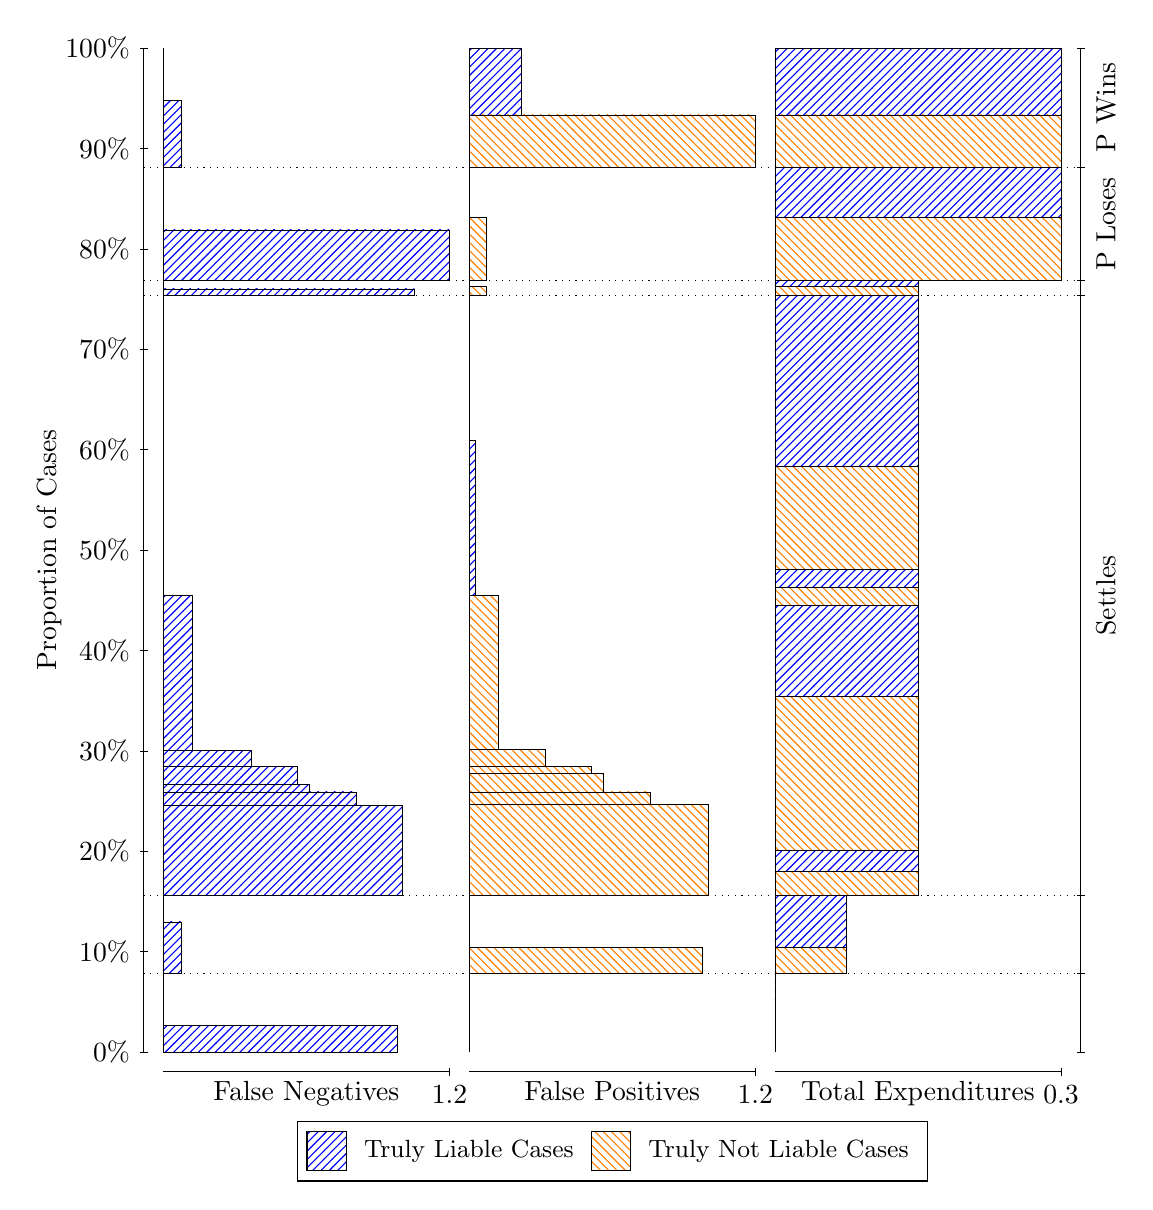
\begin{tikzpicture}
\draw[black, very thin] (1.5,1.75) -- (1.5,14.5);
\node[rotate=90, anchor=center] at (0.3, 8.125) {Proportion of Cases};
\draw[black, very thin] (1.45,1.75) -- (1.55,1.75);
\node[anchor=east] at (1.45, 1.75) {0\%};
\draw[black, very thin] (1.45,3.025) -- (1.55,3.025);
\node[anchor=east] at (1.45, 3.025) {10\%};
\draw[black, very thin] (1.45,4.3) -- (1.55,4.3);
\node[anchor=east] at (1.45, 4.3) {20\%};
\draw[black, very thin] (1.45,5.575) -- (1.55,5.575);
\node[anchor=east] at (1.45, 5.575) {30\%};
\draw[black, very thin] (1.45,6.85) -- (1.55,6.85);
\node[anchor=east] at (1.45, 6.85) {40\%};
\draw[black, very thin] (1.45,8.125) -- (1.55,8.125);
\node[anchor=east] at (1.45, 8.125) {50\%};
\draw[black, very thin] (1.45,9.4) -- (1.55,9.4);
\node[anchor=east] at (1.45, 9.4) {60\%};
\draw[black, very thin] (1.45,10.675) -- (1.55,10.675);
\node[anchor=east] at (1.45, 10.675) {70\%};
\draw[black, very thin] (1.45,11.95) -- (1.55,11.95);
\node[anchor=east] at (1.45, 11.95) {80\%};
\draw[black, very thin] (1.45,13.225) -- (1.55,13.225);
\node[anchor=east] at (1.45, 13.225) {90\%};
\draw[black, very thin] (1.45,14.5) -- (1.55,14.5);
\node[anchor=east] at (1.45, 14.5) {100\%};

\draw[black, very thin] (13.4,1.75) -- (13.4,14.5);
\draw[black, very thin] (13.35,1.75) -- (13.45,1.75);
\node[anchor=west] at (13.35, 1.75) {};
\draw[black, very thin] (13.35,2.7449) -- (13.45,2.7449);
\node[anchor=west] at (13.35, 2.7449) {};
\draw[black, very thin] (13.35,3.7383) -- (13.45,3.7383);
\node[anchor=west] at (13.35, 3.7383) {};
\draw[black, very thin] (13.35,11.358) -- (13.45,11.358);
\node[anchor=west] at (13.35, 11.358) {};
\draw[black, very thin] (13.35,11.551) -- (13.45,11.551);
\node[anchor=west] at (13.35, 11.551) {};
\draw[black, very thin] (13.35,12.984) -- (13.45,12.984);
\node[anchor=west] at (13.35, 12.984) {};
\draw[black, very thin] (13.35,14.5) -- (13.45,14.5);
\node[anchor=west] at (13.35, 14.5) {};

\draw[black, very thin, pattern color=blue, pattern=north east lines] (1.75,1.75) rectangle (4.716,2.0858);
\draw[black, very thin, pattern color=orange, pattern=north west lines] (1.75,2.0858) rectangle (1.75,2.7449);
\draw[black, very thin, pattern color=blue, pattern=north east lines] (1.75,2.7449) rectangle (1.9724,3.4033);
\draw[black, very thin, pattern color=orange, pattern=north west lines] (1.75,3.4033) rectangle (1.75,3.7383);
\draw[black, very thin, pattern color=blue, pattern=north east lines] (1.75,3.7383) rectangle (4.7901,4.8855);
\draw[black, very thin, pattern color=blue, pattern=north east lines] (1.75,4.8855) rectangle (4.1969,5.0541);
\draw[black, very thin, pattern color=blue, pattern=north east lines] (1.75,5.0541) rectangle (3.6037,5.1516);
\draw[black, very thin, pattern color=blue, pattern=north east lines] (1.75,5.1516) rectangle (3.4554,5.3808);
\draw[black, very thin, pattern color=blue, pattern=north east lines] (1.75,5.3808) rectangle (2.8622,5.5803);
\draw[black, very thin, pattern color=blue, pattern=north east lines] (1.75,5.5803) rectangle (2.1207,7.548);
\draw[black, very thin, pattern color=orange, pattern=north west lines] (1.75,7.548) rectangle (1.75,11.358);
\draw[black, very thin, pattern color=blue, pattern=north east lines] (1.75,11.358) rectangle (4.9384,11.44);
\draw[black, very thin, pattern color=orange, pattern=north west lines] (1.75,11.44) rectangle (1.75,11.551);
\draw[black, very thin, pattern color=blue, pattern=north east lines] (1.75,11.551) rectangle (5.3833,12.19);
\draw[black, very thin, pattern color=orange, pattern=north west lines] (1.75,12.19) rectangle (1.75,12.984);
\draw[black, very thin, pattern color=blue, pattern=north east lines] (1.75,12.984) rectangle (1.9724,13.834);
\draw[black, very thin, pattern color=orange, pattern=north west lines] (1.75,13.834) rectangle (1.75,14.5);
\draw[black, very thin, pattern color=orange, pattern=north west lines] (5.6333,1.75) rectangle (5.6333,2.4091);
\draw[black, very thin, pattern color=blue, pattern=north east lines] (5.6333,2.4091) rectangle (5.6333,2.7449);
\draw[black, very thin, pattern color=orange, pattern=north west lines] (5.6333,2.7449) rectangle (8.5993,3.0799);
\draw[black, very thin, pattern color=blue, pattern=north east lines] (5.6333,3.0799) rectangle (5.6333,3.7383);
\draw[black, very thin, pattern color=orange, pattern=north west lines] (5.6333,3.7383) rectangle (8.6735,4.8914);
\draw[black, very thin, pattern color=orange, pattern=north west lines] (5.6333,4.8914) rectangle (7.932,5.0541);
\draw[black, very thin, pattern color=orange, pattern=north west lines] (5.6333,5.0541) rectangle (7.3388,5.2832);
\draw[black, very thin, pattern color=orange, pattern=north west lines] (5.6333,5.2832) rectangle (7.1905,5.381);
\draw[black, very thin, pattern color=orange, pattern=north west lines] (5.6333,5.381) rectangle (6.5973,5.5888);
\draw[black, very thin, pattern color=orange, pattern=north west lines] (5.6333,5.5888) rectangle (6.0041,7.5484);
\draw[black, very thin, pattern color=blue, pattern=north east lines] (5.6333,7.5484) rectangle (5.7075,9.5161);
\draw[black, very thin, pattern color=blue, pattern=north east lines] (5.6333,9.5161) rectangle (5.6333,11.358);
\draw[black, very thin, pattern color=orange, pattern=north west lines] (5.6333,11.358) rectangle (5.8558,11.469);
\draw[black, very thin, pattern color=blue, pattern=north east lines] (5.6333,11.469) rectangle (5.6333,11.551);
\draw[black, very thin, pattern color=orange, pattern=north west lines] (5.6333,11.551) rectangle (5.8558,12.345);
\draw[black, very thin, pattern color=blue, pattern=north east lines] (5.6333,12.345) rectangle (5.6333,12.984);
\draw[black, very thin, pattern color=orange, pattern=north west lines] (5.6333,12.984) rectangle (9.2667,13.65);
\draw[black, very thin, pattern color=blue, pattern=north east lines] (5.6333,13.65) rectangle (6.3007,14.5);
\draw[black, very thin, pattern color=orange, pattern=north west lines] (9.5167,1.75) rectangle (9.5167,2.4091);
\draw[black, very thin, pattern color=blue, pattern=north east lines] (9.5167,2.4091) rectangle (9.5167,2.7449);
\draw[black, very thin, pattern color=orange, pattern=north west lines] (9.5167,2.7449) rectangle (10.425,3.0799);
\draw[black, very thin, pattern color=blue, pattern=north east lines] (9.5167,3.0799) rectangle (10.425,3.7383);
\draw[black, very thin, pattern color=orange, pattern=north west lines] (9.5167,3.7383) rectangle (11.333,4.044);
\draw[black, very thin, pattern color=blue, pattern=north east lines] (9.5167,4.044) rectangle (11.333,4.3101);
\draw[black, very thin, pattern color=orange, pattern=north west lines] (9.5167,4.3101) rectangle (11.333,6.2697);
\draw[black, very thin, pattern color=blue, pattern=north east lines] (9.5167,6.2697) rectangle (11.333,7.4168);
\draw[black, very thin, pattern color=orange, pattern=north west lines] (9.5167,7.4168) rectangle (11.333,7.646);
\draw[black, very thin, pattern color=blue, pattern=north east lines] (9.5167,7.646) rectangle (11.333,7.8751);
\draw[black, very thin, pattern color=orange, pattern=north west lines] (9.5167,7.8751) rectangle (11.333,9.1908);
\draw[black, very thin, pattern color=blue, pattern=north east lines] (9.5167,9.1908) rectangle (11.333,11.358);
\draw[black, very thin, pattern color=orange, pattern=north west lines] (9.5167,11.358) rectangle (11.333,11.469);
\draw[black, very thin, pattern color=blue, pattern=north east lines] (9.5167,11.469) rectangle (11.333,11.551);
\draw[black, very thin, pattern color=orange, pattern=north west lines] (9.5167,11.551) rectangle (13.15,12.345);
\draw[black, very thin, pattern color=blue, pattern=north east lines] (9.5167,12.345) rectangle (13.15,12.984);
\draw[black, very thin, pattern color=orange, pattern=north west lines] (9.5167,12.984) rectangle (13.15,13.65);
\draw[black, very thin, pattern color=blue, pattern=north east lines] (9.5167,13.65) rectangle (13.15,14.5);
\draw[black, dotted] (1.5,2.7449) -- (13.4,2.7449);
\draw[black, dotted] (1.5,3.7383) -- (13.4,3.7383);
\draw[black, dotted] (1.5,11.358) -- (13.4,11.358);
\draw[black, dotted] (1.5,11.551) -- (13.4,11.551);
\draw[black, dotted] (1.5,12.984) -- (13.4,12.984);
\draw[black, very thin] (1.75,1.5) -- (5.3833,1.5);
\node[anchor=north] at (3.5667, 1.5) {False Negatives};
\draw[black, very thin] (5.3833,1.45) -- (5.3833,1.55);
\node[anchor=north] at (5.3833, 1.45) {1.2};

\draw[black, very thin] (5.6333,1.5) -- (9.2667,1.5);
\node[anchor=north] at (7.45, 1.5) {False Positives};
\draw[black, very thin] (9.2667,1.45) -- (9.2667,1.55);
\node[anchor=north] at (9.2667, 1.45) {1.2};

\draw[black, very thin] (9.5167,1.5) -- (13.15,1.5);
\node[anchor=north] at (11.333, 1.5) {Total Expenditures};
\draw[black, very thin] (13.15,1.45) -- (13.15,1.55);
\node[anchor=north] at (13.15, 1.45) {0.3};



\node[black, centered, rotate=90] at (13.72, 7.5482) {Settles};

\node[black, centered, rotate=90] at (13.72, 12.267) {P Loses};
\node[black, centered, rotate=90] at (13.72, 13.742) {P Wins};

\draw (7.449999999999999,1.5) node[draw=none] (baseCoordinate) {};
\begin{scope}[align=center]
        \matrix[scale=0.5, draw=black, below=0.5cm of baseCoordinate, nodes={draw}, column sep=0.1cm]{
            \node[rectangle, draw, minimum width=0.5cm, minimum height=0.5cm, pattern=north east lines, pattern color=blue] {}; &
            \node[draw=none, font=\small] (B) {Truly Liable Cases}; &
            \node[rectangle, draw, minimum width=0.5cm, minimum height=0.5cm, pattern=north west lines, pattern color=orange] {}; &
            \node[draw=none, font=\small] (B) {Truly Not Liable Cases}; \\
            };
\end{scope}

\end{tikzpicture}
\end{document}